\documentclass[./main.tex]{subfiles}

\begin{document}
\section{Introduction}
\begin{figure}[htbp]
    \centering
    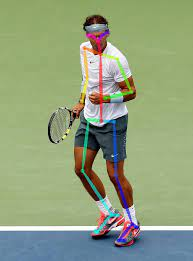
\includegraphics[height = 6 cm]{./entities/pose_estimation_example_img.jpg}
    \caption{Example of 2D single-person articulated human pose estimation \cite{pose_estimation_example}}
    \label{fig:pose_estimation_example_fig}
\end{figure}
% Real-world applications
\noindent It is common knowledge, that the real-world use of artificial intelligence and machine learning is growing rapidly. With this growth the need for accurate computer vision models is also increasing. One usage of computer vision is \textit{2D human pose estimation}, where a machine learning model is used for estimating the pose of one, or multiple, humans. These models have many real-world applications, such as motion analysis, augmented reality and virtual reality \cite{survey_2}.
\\
\\
% Describing pose estimation
The goal of human pose estimation is to estimate the pose of one or multiple humans in images or videos. There are different types of human pose estimations, where one of the most common ones is the \textit{articulated} human pose estimation, which is done by estimating the location of various keypoints of the human bodies in an input. The methods within human pose estimation can further be split into $2D$ human pose estimation and $3D$ human pose estimation, which describes the amount of dimensions in the estimations. An example of a $2$D articulated human pose estimation of a single person has been visualized in Figure \ref{fig:pose_estimation_example_fig}.
\\
\\
% Motivation for XAI
As the complexity of machine learning models have increased, the models have started to work more and more as a "black box", where it can be difficult to understand how the models work and why they work as they do. This can lead to problems such as distrust, redundancy or difficulty with improving the performance of the models \cite{Selvaraju}.
\\
\\
% Problem statement/thesis goals
The goal of this thesis is thus to select a model for human pose estimation, to interpretate the developed model, as well as use the obtained knowledge about the model to modify and improve the model. % Mangler at beskrive/argumentere valg af model
\\
\\
% Structure of thesis
In the remainder of this thesis, Section \ref{sec:theory} introduces the basic machine learning theory and Section \ref{sec:algorithms} introduces the most important algortihms used throughout the thesis. In Section \ref{sec:dataset} the used dataset and its preprocessing is described. We then describe our development of a model and its respective results in Section \ref{experiement}, which is then explored and interpreted in Section \ref{sec:XAI}. In Section \ref{sec:improving}, we then use our knowledge of the model to improve the performance of it. We then discuss our approach and results in Section \ref{sec:discussion}. Lastly, we conclude our results in Section \ref{sec:conclusion}.

\end{document}